\documentclass[11pt,pdftex,aspectratio=1610]{beamer}
\usepackage{amsmath, amsthm, amssymb}
\usepackage{color}
\usepackage{hyperref}
\usepackage{subfigure}
\usepackage{tabularx}
\usepackage{ragged2e}
\usepackage{booktabs}
\usepackage{multirow}
\usepackage{bbm}
\usepackage[listings, most]{tcolorbox}

\usecolortheme{dolphin}
\linespread{1.3}
\definecolor{nblue}{RGB}{0,0,128}

\setbeamercovered{transparent}

\newcolumntype{Y}{>{\RaggedRight\arraybackslash}X}

\hypersetup{colorlinks=true, linkcolor=nblue,
citecolor=nblue, urlcolor=nblue, bookmarks=false,
pdfpagemode=UseNone,
pdfstartview={XYZ null null 1.0},
pdftitle={Trade in AI-Related Products},
pdfauthor={Michael E. Waugh},
pdfkeywords={AI, trade, data centers, tariffs, imports, exports, HS10, LLM classification}}

\setbeamertemplate{navigation symbols}{}
\setbeamertemplate{footline}[frame number]
\setbeamertemplate{theorems}[numbered]
\setbeamertemplate{itemize subitem}[circle]
\setbeamertemplate{enumerate items}[default]

\setbeamerfont{frametitle}{size= \large}
\setbeamerfont{ framesubtitle }{size = \footnotesize}
\setbeamertemplate{frametitle}
{
\medskip
\smallskip
{\textsf{\underline{\insertframetitle\phantom{))))))))}}}}}
\setbeamertemplate{items}[circle]
\setbeamertemplate{itemize subitem}[circle]

\usepackage[normalem]{ulem}
\newcommand\redout{\bgroup\markoverwith
{\textcolor{red}{\rule[.5ex]{1pt}{1pt}}}\ULon}

\makeatletter
\def\blfootnote{\xdef\@thefnmark{}\@footnotetext}
\makeatother

% Load the computed macros from the paper pipeline
\def\highAiHsCodes{645} % Number of HS10 codes classified as high AI relevance
\def\highAiTwentyThree{379} % High AI relevance imports in 2023 ($B)
\def\highAiTwentyFive{654} % High AI relevance imports in 2025 ($B)
\def\highAiPctChange{73} % High AI relevance percent change 2023-2025
\def\lowAiHsCodes{15915} % Number of HS10 codes classified as low AI relevance
\def\lowAiTwentyThree{1835} % Low AI relevance imports in 2023 ($B)
\def\lowAiTwentyFive{1881} % Low AI relevance imports in 2025 ($B)
\def\lowAiPctChange{3} % Low AI relevance percent change 2023-2025
\def\totalTradeHsCodes{18364} % Total number of HS10 codes in dataset
\def\totalTradeTwentyThree{2598} % Total imports in 2023 ($B)
\def\totalTradeTwentyFive{2884} % Total imports in 2025 ($B)
\def\totalTradePctChange{11} % Total trade percent change 2023-2025
\newcommand{\ComputeHardwareHsCodes}{163} % Number of HS10 codes in Compute Hardware
\newcommand{\ComputeHardwareTwentyThree}{144} % Compute Hardware imports in 2023 ($B)
\newcommand{\ComputeHardwareTwentyFive}{354} % Compute Hardware imports in 2025 ($B)
\newcommand{\ComputeHardwarePctChange}{145} % Compute Hardware percent change 2023-2025
\newcommand{\ElectricalPowerHsCodes}{250} % Number of HS10 codes in Electrical Power
\newcommand{\ElectricalPowerTwentyThree}{117} % Electrical Power imports in 2023 ($B)
\newcommand{\ElectricalPowerTwentyFive}{142} % Electrical Power imports in 2025 ($B)
\newcommand{\ElectricalPowerPctChange}{21} % Electrical Power percent change 2023-2025
\newcommand{\NetworkingTelecomHsCodes}{24} % Number of HS10 codes in Networking Telecom
\newcommand{\NetworkingTelecomTwentyThree}{63} % Networking Telecom imports in 2023 ($B)
\newcommand{\NetworkingTelecomTwentyFive}{100} % Networking Telecom imports in 2025 ($B)
\newcommand{\NetworkingTelecomPctChange}{58} % Networking Telecom percent change 2023-2025
\newcommand{\CoolingHVACHsCodes}{137} % Number of HS10 codes in Cooling HVAC
\newcommand{\CoolingHVACTwentyThree}{42} % Cooling HVAC imports in 2023 ($B)
\newcommand{\CoolingHVACTwentyFive}{48} % Cooling HVAC imports in 2025 ($B)
\newcommand{\CoolingHVACPctChange}{14} % Cooling HVAC percent change 2023-2025
\newcommand{\BuildingStructureHsCodes}{44} % Number of HS10 codes in Building Structure
\newcommand{\BuildingStructureTwentyThree}{12} % Building Structure imports in 2023 ($B)
\newcommand{\BuildingStructureTwentyFive}{10} % Building Structure imports in 2025 ($B)
\newcommand{\BuildingStructurePctChange}{-16} % Building Structure percent change 2023-2025
\newcommand{\FireSafetySecurityHsCodes}{8} % Number of HS10 codes in Fire Safety Security
\newcommand{\FireSafetySecurityTwentyThree}{1} % Fire Safety Security imports in 2023 ($B)
\newcommand{\FireSafetySecurityTwentyFive}{1} % Fire Safety Security imports in 2025 ($B)
\newcommand{\FireSafetySecurityPctChange}{10} % Fire Safety Security percent change 2023-2025
\newcommand{\SpecialtyMaterialsHsCodes}{19} % Number of HS10 codes in Specialty Materials
\newcommand{\SpecialtyMaterialsTwentyThree}{0} % Specialty Materials imports in 2023 ($B)
\newcommand{\SpecialtyMaterialsTwentyFive}{0} % Specialty Materials imports in 2025 ($B)
\newcommand{\SpecialtyMaterialsPctChange}{23} % Specialty Materials percent change 2023-2025
\def\totalHighAiHsCodes{645} % Total HS10 codes across all high AI categories
\def\totalHighAiTwentyThree{379} % Total high AI imports in 2023 ($B)
\def\totalHighAiTwentyFive{654} % Total high AI imports in 2025 ($B)
\def\totalHighAiPctChange{73} % Total high AI percent change 2023-2025
\def\aiRelevantIndex{211} % AI-relevant imports index (2023=100)
\def\aggregateIndex{104} % Aggregate imports index (2023=100)
\def\notAiRelevantIndex{86} % Non-AI-relevant imports index (2023=100)
\def\lastObsDate{January 2026} % Last observation date
\def\aiRelevantGrowth{111} % AI-relevant imports growth vs 2023 (%)
\def\notAiRelevantDecline{14} % Non-AI-relevant imports decline vs 2023 (%)
\def\aiShareTwentyThree{15} % AI share of total imports in 2023 (%)
\def\aiShareTwentyFour{17} % AI share of total imports in 2024 (%)
\def\aiShareTwentyFive{23} % AI share of total imports in 2025 (%)
\def\aiShareGrowth{8} % AI share growth 2023-2025 (percentage points)
\def\canadaHighAiImportGrowthTwentyFiveVsTwentyFour{-4.2} % Canada high-AI import growth in 2025 vs 2024 (%)
\def\mexicoHighAiImportGrowthTwentyFiveVsTwentyFour{40.7} % Mexico high-AI import growth in 2025 vs 2024 (%)
\def\canadaTotalImportGrowthTwentyFiveVsTwentyFour{-8.3} % Canada total import growth in 2025 vs 2024 (%)
\def\mexicoTotalImportGrowthTwentyFiveVsTwentyFour{6.4} % Mexico total import growth in 2025 vs 2024 (%)
\def\mexicoLowAiImportGrowthTwentyFiveVsTwentyFour{-4.2} % Mexico non-AI import growth in 2025 vs 2024 (%)
\def\tariffHighTwentyFour{1.8} % High AI relevance tariff rate in 2024 (%)
\def\tariffHighTwentyFive{4.5} % High AI relevance tariff rate in Dec 2025 (%)
\def\tariffLowTwentyFour{2.7} % Low AI relevance tariff rate in 2024 (%)
\def\tariffLowTwentyFive{12.1} % Low AI relevance tariff rate in Dec 2025 (%)
\newcommand{\tariffComputeHardwareTwentyFour}{0.6} % Compute Hardware tariff rate in 2024 (%)
\newcommand{\tariffComputeHardwareTwentyFive}{0.8} % Compute Hardware tariff rate in Dec 2025 (%)
\newcommand{\tariffElectricalPowerTwentyFour}{3.5} % Electrical Power tariff rate in 2024 (%)
\newcommand{\tariffElectricalPowerTwentyFive}{13.8} % Electrical Power tariff rate in Dec 2025 (%)
\newcommand{\tariffNetworkingTelecomTwentyFour}{1.5} % Networking Telecom tariff rate in 2024 (%)
\newcommand{\tariffNetworkingTelecomTwentyFive}{3.1} % Networking Telecom tariff rate in Dec 2025 (%)
\newcommand{\tariffCoolingHVACTwentyFour}{3.0} % Cooling HVAC tariff rate in 2024 (%)
\newcommand{\tariffCoolingHVACTwentyFive}{15.8} % Cooling HVAC tariff rate in Dec 2025 (%)
\def\exemptionAnyPct{69} % Share of AI High imports on any exemption list (%)
\def\exemptionCEDollars{424} % Consumer Electronics exemption coverage ($B)
\def\exemptionComputeHardwarePct{97.3} % Compute Hardware exemption coverage (%)
\def\exemptionElectricalPowerPct{13.5} % Electrical Power exemption coverage (%)
\def\exemptionNetworkingTelecomPct{85.1} % Networking Telecom exemption coverage (%)
\def\exemptionCoolingHVACPct{0.4} % Cooling HVAC exemption coverage (%)
\def\exemptionBuildingStructurePct{0.0} % Building Structure exemption coverage (%)
\def\exemptionFireSafetySecurityPct{0.0} % Fire Safety Security exemption coverage (%)
\def\exemptionSpecialtyMaterialsPct{60.8} % Specialty Materials exemption coverage (%)
\def\aiExportGrowth{34.5} % AI-related export growth 2023-2025 (%)
\newcommand{\computeHardwareExportGrowth}{62.1} % Compute Hardware export growth 2023-2025 (%)
\def\cfExcessAiImports{265}
\def\cfExcessAiExports{71}
\def\cfNetAiEffect{194}
\def\cfActualBalance{-1235}
\def\cfCounterfactualBalance{-1041}
\def\cfActualDeficit{1,235} % Actual goods trade deficit 2025 ($B)
\def\cfCounterfactualDeficit{1,041} % Counterfactual goods trade deficit 2025 ($B)
\def\cfDeficitReductionPct{16} % Deficit reduction from AI boom (%)


% Counterfactual macros (from notebook 11, not in ai-trade-results.tex)
\def\cfNetAiEffect{194}

%%%%%%%%%%%%%%%%%%%%%%%%%%%%%%%%%%%%%%%%%%%%%%%%%%%%%%%%%%%%%%%%%%%%%%%%%%%%%%%%%%%%%%%%%%%%%%%%%
%%%%%%%%%%%%%%%%%%%%%%%%%%%%%%%%%%%%%%%%%%%%%%%%%%%%%%%%%%%%%%%%%%%%%%%%%%%%%%%%%%%%%%%%%%%%%%%%%

\title{\Large Trade in AI-Related Products}
\institute[Foo and Bar]{\normalsize\begin{tabular}[h]{c}
Michael E. Waugh  \\
Federal Reserve Bank of Minneapolis\blfootnote{The views expressed herein are those of the author and not necessarily those of the Federal
Reserve Bank of Minneapolis or the Federal Reserve System.} and NBER\\
\href{https://twitter.com/tradewartracker}{@tradewartracker}
\end{tabular}}

\date{March 2026}

\begin{document}

\begin{frame}
\titlepage
\setcounter{framenumber}{0}
\section{}
\end{frame}

%%%%%%%%%%%%%%%%%%%%%%%%%%%%%%%%%%%%%%%%%%%%%%%%%%%%%%%%%%%%%%%%%%%%%%%%%%%%%%%%%%%%%%%%%%%%%%%%%
%%%%%%%%%%%%%%%%%%%%%%%%%%%%%%%%%%%%%%%%%%%%%%%%%%%%%%%%%%%%%%%%%%%%%%%%%%%%%%%%%%%%%%%%%%%%%%%%%

\begin{frame}[t]{The AI Infrastructure Boom and Trade}
\smallskip
The U.S. is experiencing a massive AI-investment-driven boom | trillions of dollars invested in data centers and related AI infrastructure.\\
\bigskip
\bigskip
\textbf{This paper asks:} How is the AI boom influencing international trade flows?\\
\bigskip
\bigskip
Trade in AI-related products is \emph{the} dominant force in U.S. trade flows over the past two years. Not changes in U.S. trade policy.\\
\bigskip
\end{frame}

%%%%%%%%%%%%%%%%%%%%%%%%%%%%%%%%%%%%%%%%%%%%%%%%%%%%%%%%%%%%%%%%%%%%%%%%%%%%%%%%%%%%%%%%%%%%%%%%%
%%%%%%%%%%%%%%%%%%%%%%%%%%%%%%%%%%%%%%%%%%%%%%%%%%%%%%%%%%%%%%%%%%%%%%%%%%%%%%%%%%%%%%%%%%%%%%%%%

\begin{frame}[t]{Six questions\ldots}
\begin{itemize}
\item How to classify AI-related products?
\medskip
\item What are AI-related products?
\medskip
\item How much trade in AI-related products?
\medskip
\item Where are these products coming from?
\medskip
\item How has trade policy treated AI-related products?
\medskip
\item Does this matter for the aggregate?
\end{itemize}
\end{frame}
%%%%%%%%%%%%%%%%%%%%%%%%%%%%%%%%%%%%%%%%%%%%%%%%%%%%%%%%%%%%%%%%%%%%%%%%%%%%%%%%%%%%%%%%%%%%%%%%%
%%%%%%%%%%%%%%%%%%%%%%%%%%%%%%%%%%%%%%%%%%%%%%%%%%%%%%%%%%%%%%%%%%%%%%%%%%%%%%%%%%%%%%%%%%%%%%%%%

\begin{frame}[t]{How to Classify AI-Related Products?}
Use an LLM to classify each of the $\sim$18,000 HS10 commodity codes by relevance to AI data center infrastructure. Snippet of the prompt:\\
{\tiny
\begin{tcolorbox}[colback=gray!5!white, colframe=gray!50!white, boxrule=0.5pt, top=3mm, bottom=3mm, left=3mm, right=3mm]
{\small \texttt{You are an expert in AI data center construction, operations, and supply chains. Your task is to classify products by their relevance to building and operating AI-focused data centers (hyperscale facilities running GPU clusters for training and inference).}\\

\texttt{Consider these categories of relevant products:}\\
\texttt{- COMPUTE: GPUs, CPUs, memory, PCBs, servers, storage drives}\\
\texttt{- NETWORKING: Fiber optics, switches, routers, transceivers}\\
\texttt{- COOLING: Chillers, cooling towers, CRAH units, fans, pumps}\\
\texttt{- ELECTRICAL: Transformers, switchgear, UPS, batteries, generators}\\
\texttt{- BUILDING: Structural steel, concrete, rebar, raised floors}\\
\texttt{- SPECIALTY MATERIALS: Rare earths, copper, aluminum\ldots}}
\end{tcolorbox}}
\medskip
{\small Each HS10 code gets: \textbf{Relevance}, \textbf{Category}, \textbf{Confidence}, and \textbf{Reasoning}.}
%\smallskip
%Uses Claude (Anthropic) with structured tool calling | schema enforcement ensures valid outputs.
\end{frame}

%%%%%%%%%%%%%%%%%%%%%%%%%%%%%%%%%%%%%%%%%%%%%%%%%%%%%%%%%%%%%%%%%%%%%%%%%%%%%%%%%%%%%%%%%%%%%%%%%
%%%%%%%%%%%%%%%%%%%%%%%%%%%%%%%%%%%%%%%%%%%%%%%%%%%%%%%%%%%%%%%%%%%%%%%%%%%%%%%%%%%%%%%%%%%%%%%%%

\begin{frame}[t]{How to Classify AI-Related Products? | An Example}
The LLM sees the HS10 description \emph{and} the NAICS industry code:\\
{\tiny
\begin{tcolorbox}[colback=gray!5!white, colframe=gray!50!white, boxrule=0.5pt, top=3mm, bottom=3mm, left=3mm, right=3mm]
{\small
\texttt{HS10: 8542310040}\\
\texttt{Description: PROCESSORS (INCLUDING MICROPROCESSORS): GRAPHICS PROCESSING UNITS (GPUS)}\\
\texttt{NAICS: 334413 --- SEMICONDUCTOR AND RELATED DEVICE MANUFACTURING}\\[6pt]
\texttt{RELEVANCE: High \quad CONFIDENCE: 100\%}\\
\texttt{CATEGORY: Compute Hardware}\\
\texttt{REASONING: GPUs are the core compute hardware in AI data centers, specifically designed for parallel processing required in ML training and inference.}
}
\end{tcolorbox}}
\bigskip
Baseline analysis focuses on products classified as \textbf{High} | those directly used in data center construction or operation.\\
\medskip
Result: \highAiHsCodes{} High-relevance codes out of \totalTradeHsCodes{} total.
\end{frame}

%%%%%%%%%%%%%%%%%%%%%%%%%%%%%%%%%%%%%%%%%%%%%%%%%%%%%%%%%%%%%%%%%%%%%%%%%%%%%%%%%%%%%%%%%%%%%%%%%
%%%%%%%%%%%%%%%%%%%%%%%%%%%%%%%%%%%%%%%%%%%%%%%%%%%%%%%%%%%%%%%%%%%%%%%%%%%%%%%%%%%%%%%%%%%%%%%%%

\begin{frame}[t]{What Are AI-Related Products?}
\smallskip
\begin{table}[t]
\centering
\setlength{\tabcolsep}{2.25mm}
\renewcommand{\arraystretch}{1.0}
\begin{tabular}{lcccc}
\toprule
Category & \# HS10 Codes & 2023 (\$B) & 2025 (\$B) & Change (\%) \\
\midrule
\textbf{High AI Relevance} & \textbf{645} & \textbf{379.0} & \textbf{654.0} & \textbf{+72.6} \\
\quad Compute Hardware & 163 & 144.4 & 353.8 & +144.9 \\
\quad Electrical Power & 250 & 116.9 & 141.8 & +21.3 \\
\quad Networking Telecom & 24 & 62.9 & 99.5 & +58.2 \\
\quad Cooling HVAC & 137 & 41.5 & 47.5 & +14.4 \\
\quad Building Structure & 44 & 12.1 & 10.1 & -16.5 \\
\quad Fire Safety Security & 8 & 0.6 & 0.7 & +10.5 \\
\quad Specialty Materials & 19 & 0.4 & 0.5 & +22.5 \\
\midrule
Low AI Relevance & 15,915 & 1,834.7 & 1,880.9 & +2.5 \\
\midrule
\textbf{Total Trade} & \textbf{18,364} & \textbf{2,598.3} & \textbf{2,883.9} & \textbf{+11.0} \\
\bottomrule
\end{tabular}
\end{table}
\end{frame}

%%%%%%%%%%%%%%%%%%%%%%%%%%%%%%%%%%%%%%%%%%%%%%%%%%%%%%%%%%%%%%%%%%%%%%%%%%%%%%%%%%%%%%%%%%%%%%%%%
%%%%%%%%%%%%%%%%%%%%%%%%%%%%%%%%%%%%%%%%%%%%%%%%%%%%%%%%%%%%%%%%%%%%%%%%%%%%%%%%%%%%%%%%%%%%%%%%%

\begin{frame}[t]{What Are AI-Related Products? | Top 10 by Import Volume}
\begin{table}[t]
\centering
\setlength{\tabcolsep}{1.0mm}
\renewcommand{\arraystretch}{1.0}
{\small
\begin{tabular}{lp{4.5cm}lccc}
\toprule
HS10 Code & Description & Category & 2025 (\$B) & Share (\%) & $\Delta$ (\%) \\
\midrule
8471500150 & Data processing units & Compute HW & 163.6 & 5.67 & +343 \\
8517620090 & Telecom transmission equip. & Network & 52.9 & 1.83 & +58 \\
8473301180 & Printed circuit assemblies & Compute HW & 48.9 & 1.70 & +200 \\
8517620020 & Switching \& routing apparatus & Network & 30.8 & 1.07 & +89 \\
8473301140 & Memory modules & Compute HW & 25.8 & 0.89 & +206 \\
8523510000 & SSDs & Compute HW & 17.5 & 0.61 & +85 \\
7403110000 & Refined copper cathodes & Electrical & 16.6 & 0.58 & +150 \\
8507600020 & Lithium-ion batteries & Electrical & 16.5 & 0.57 & +11 \\
8537109170 & Electrical switchgear & Electrical & 11.3 & 0.39 & +13 \\
8471804000 & Units for ADP machines & Compute HW & 11.1 & 0.39 & +937 \\
\bottomrule
\end{tabular}}
\end{table}
\smallskip
All ten products show double-digit growth; five show \begin{alert}{\textbf{triple-digit}}\end{alert} growth since 2023.
\end{frame}

%%%%%%%%%%%%%%%%%%%%%%%%%%%%%%%%%%%%%%%%%%%%%%%%%%%%%%%%%%%%%%%%%%%%%%%%%%%%%%%%%%%%%%%%%%%%%%%%%
%%%%%%%%%%%%%%%%%%%%%%%%%%%%%%%%%%%%%%%%%%%%%%%%%%%%%%%%%%%%%%%%%%%%%%%%%%%%%%%%%%%%%%%%%%%%%%%%%

\begin{frame}[t]{How Much Trade in AI-Related Products? A lot.}
\begin{figure}[t]
\centerline{
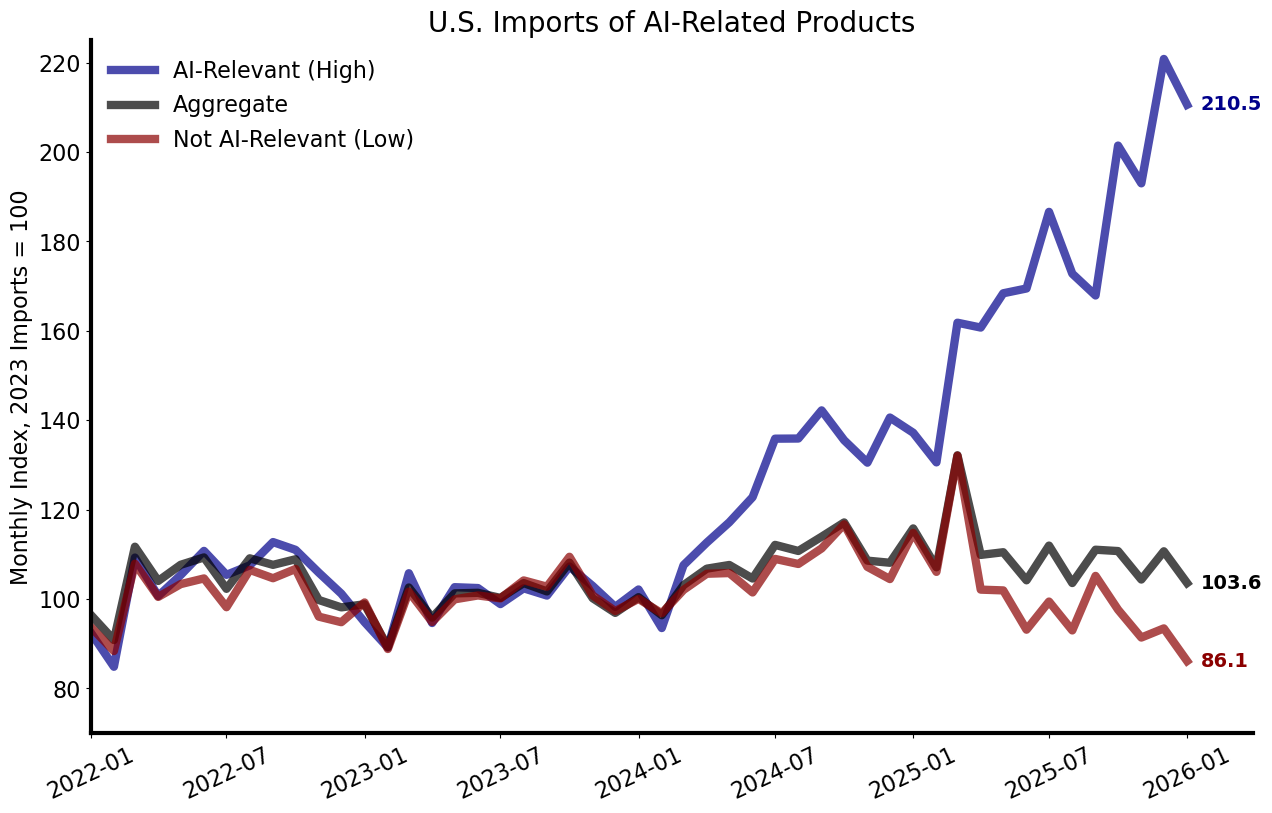
\includegraphics[scale = 0.4]{../paper/figures/ai-trade-index.pdf}}
\end{figure}
\end{frame}

%%%%%%%%%%%%%%%%%%%%%%%%%%%%%%%%%%%%%%%%%%%%%%%%%%%%%%%%%%%%%%%%%%%%%%%%%%%%%%%%%%%%%%%%%%%%%%%%%
%%%%%%%%%%%%%%%%%%%%%%%%%%%%%%%%%%%%%%%%%%%%%%%%%%%%%%%%%%%%%%%%%%%%%%%%%%%%%%%%%%%%%%%%%%%%%%%%%

\begin{frame}[t]{How Much Trade in AI-Related Products? | Share of Imports}
\begin{figure}[t]
\centerline{

\includegraphics[scale = 0.45]{../paper/figures/ai-trade-share.pdf}}
\end{figure}
\end{frame}

%%%%%%%%%%%%%%%%%%%%%%%%%%%%%%%%%%%%%%%%%%%%%%%%%%%%%%%%%%%%%%%%%%%%%%%%%%%%%%%%%%%%%%%%%%%%%%%%%
%%%%%%%%%%%%%%%%%%%%%%%%%%%%%%%%%%%%%%%%%%%%%%%%%%%%%%%%%%%%%%%%%%%%%%%%%%%%%%%%%%%%%%%%%%%%%%%%%

\begin{frame}[t]{Where Are These Products Coming From? Mexico and Taiwan}
\begin{figure}[t]
\centerline{

\includegraphics[scale = 0.45]{../paper/figures/ai-by-country.pdf}}
\end{figure}
\end{frame}

%%%%%%%%%%%%%%%%%%%%%%%%%%%%%%%%%%%%%%%%%%%%%%%%%%%%%%%%%%%%%%%%%%%%%%%%%%%%%%%%%%%%%%%%%%%%%%%%%
%%%%%%%%%%%%%%%%%%%%%%%%%%%%%%%%%%%%%%%%%%%%%%%%%%%%%%%%%%%%%%%%%%%%%%%%%%%%%%%%%%%%%%%%%%%%%%%%%

\begin{frame}[t]{Where Are These Products Coming From? | By Category}
\begin{figure}[t]
\centerline{

\includegraphics[scale = 0.45]{../paper/figures/ai-by-country-category.pdf}}
\end{figure}
\end{frame}

%%%%%%%%%%%%%%%%%%%%%%%%%%%%%%%%%%%%%%%%%%%%%%%%%%%%%%%%%%%%%%%%%%%%%%%%%%%%%%%%%%%%%%%%%%%%%%%%%
%%%%%%%%%%%%%%%%%%%%%%%%%%%%%%%%%%%%%%%%%%%%%%%%%%%%%%%%%%%%%%%%%%%%%%%%%%%%%%%%%%%%%%%%%%%%%%%%%

\begin{frame}[t]{How Has Trade Policy Treated AI-Related Products? Lightly.}
\begin{figure}[t]
\centerline{

\includegraphics[scale = 0.45]{../paper/figures/ai-tariffs.pdf}}
\end{figure}
\end{frame}

%%%%%%%%%%%%%%%%%%%%%%%%%%%%%%%%%%%%%%%%%%%%%%%%%%%%%%%%%%%%%%%%%%%%%%%%%%%%%%%%%%%%%%%%%%%%%%%%%
%%%%%%%%%%%%%%%%%%%%%%%%%%%%%%%%%%%%%%%%%%%%%%%%%%%%%%%%%%%%%%%%%%%%%%%%%%%%%%%%%%%%%%%%%%%%%%%%%

\begin{frame}[t]{How Has Trade Policy Treated AI-Related Products? | Exemptions}
\begin{table}[t]
\centering
\setlength{\tabcolsep}{1.5mm}
\renewcommand{\arraystretch}{1.25}
\begin{tabular}{lccc}
\toprule
Exemption List & \# HS10 Codes & AI High Trade (\$B) & Share (\%) \\
\midrule
Consumer Electronics (EO 14257) & 109 & 424.5 & 64.9 \\
Annex II (EO 14257) & 720 & 19.4 & 3.0 \\
Section 122 Surcharge (Feb 2026) & 1,098 & 445.9 & 68.2 \\
\midrule
\textbf{Any Exemption List} & --- & \textbf{448.6} & \textbf{68.6} \\
\bottomrule
\end{tabular}
\end{table}
\medskip
Nearly \begin{alert}{\textbf{69\%}}\end{alert} of AI-related imports by value fall on at least one exemption list. Compute Hardware is almost entirely shielded | 97\% of its \$354B in imports is exempt.
\end{frame}

%%%%%%%%%%%%%%%%%%%%%%%%%%%%%%%%%%%%%%%%%%%%%%%%%%%%%%%%%%%%%%%%%%%%%%%%%%%%%%%%%%%%%%%%%%%%%%%%%
%%%%%%%%%%%%%%%%%%%%%%%%%%%%%%%%%%%%%%%%%%%%%%%%%%%%%%%%%%%%%%%%%%%%%%%%%%%%%%%%%%%%%%%%%%%%%%%%%

\begin{frame}[t]{U.S. Exports of AI-Related Products}
\smallskip
The export side tells a complementary story | U.S. exporters play an important role in the global AI value chain.\\
\bigskip
\begin{table}[t]
\centering
\setlength{\tabcolsep}{2.0mm}
\renewcommand{\arraystretch}{1.05}
\begin{tabular}{lcccc}
\toprule
Category & \# HS10 Codes & 2023 (\$B) & 2025 (\$B) & Change (\%) \\
\midrule
\textbf{High AI Relevance} & \textbf{534} & \textbf{221.5} & \textbf{297.9} & \textbf{+34.5} \\
\quad Compute Hardware & 112 & 99.1 & 160.6 & +62.1 \\
\quad Electrical Power & 219 & 64.5 & 70.1 & +8.8 \\
\quad Networking Telecom & 23 & 29.1 & 37.7 & +29.7 \\
\quad Cooling HVAC & 128 & 24.1 & 25.0 & +3.5 \\
\midrule
Low AI Relevance & 8,278 & 1,034.8 & 1,058.6 & +2.3 \\
\midrule
\textbf{Total Trade} & \textbf{9,269} & \textbf{1,551.9} & \textbf{1,648.4} & \textbf{+6.2} \\
\bottomrule
\end{tabular}
\end{table}
\end{frame}

%%%%%%%%%%%%%%%%%%%%%%%%%%%%%%%%%%%%%%%%%%%%%%%%%%%%%%%%%%%%%%%%%%%%%%%%%%%%%%%%%%%%%%%%%%%%%%%%%
%%%%%%%%%%%%%%%%%%%%%%%%%%%%%%%%%%%%%%%%%%%%%%%%%%%%%%%%%%%%%%%%%%%%%%%%%%%%%%%%%%%%%%%%%%%%%%%%%

\begin{frame}[t]{U.S. Exports of AI-Related Products}
\begin{figure}[t]
\centerline{
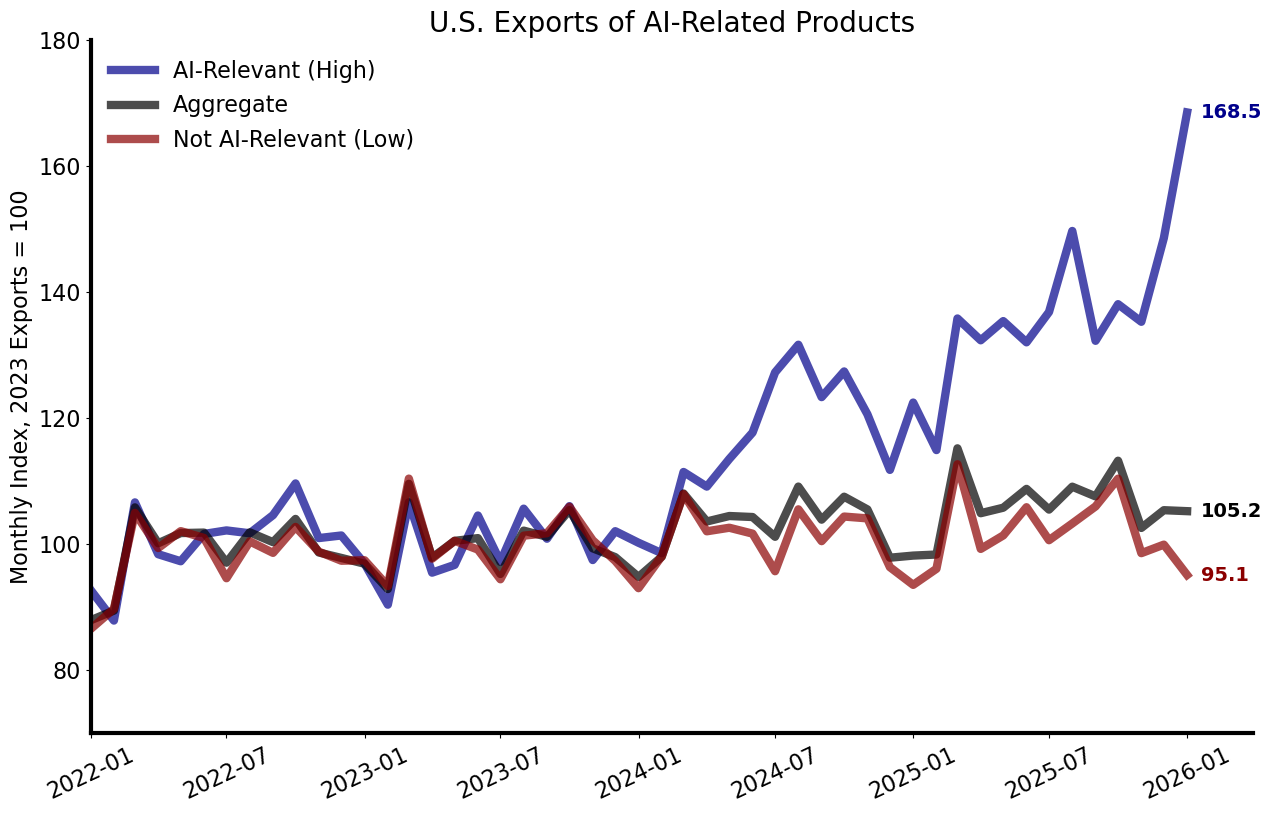
\includegraphics[scale = 0.40]{../paper/figures/ai-exports-index.pdf}}
\end{figure}
\end{frame}

%%%%%%%%%%%%%%%%%%%%%%%%%%%%%%%%%%%%%%%%%%%%%%%%%%%%%%%%%%%%%%%%%%%%%%%%%%%%%%%%%%%%%%%%%%%%%%%%%
%%%%%%%%%%%%%%%%%%%%%%%%%%%%%%%%%%%%%%%%%%%%%%%%%%%%%%%%%%%%%%%%%%%%%%%%%%%%%%%%%%%%%%%%%%%%%%%%%

\begin{frame}[t]{U.S. Exports of AI-Related Products | Destinations}
\begin{figure}[t]
\centerline{
\includegraphics[scale = 0.35]{../paper/figures/ai-exports-by-country-category.pdf}}
\end{figure}
Mexico is an important \emph{destination} for AI-related exports | suggestive that AI materials come into the U.S., go to Mexico, and back.
\end{frame}

%%%%%%%%%%%%%%%%%%%%%%%%%%%%%%%%%%%%%%%%%%%%%%%%%%%%%%%%%%%%%%%%%%%%%%%%%%%%%%%%%%%%%%%%%%%%%%%%%
%%%%%%%%%%%%%%%%%%%%%%%%%%%%%%%%%%%%%%%%%%%%%%%%%%%%%%%%%%%%%%%%%%%%%%%%%%%%%%%%%%%%%%%%%%%%%%%%%

\begin{frame}[t]{Does This Matter for the Aggregate? Yes.}
\smallskip
A simple accounting exercise:\\
\smallskip
What would the U.S. goods trade deficit have been if AI-related products had grown the same as non-AI products?\\
\bigskip
\begin{table}[t]
\centering
\setlength{\tabcolsep}{2.25mm}
\renewcommand{\arraystretch}{1.30}
\begin{tabular}{lccccc}
\toprule
Year & Imports & Exports & Excess AI Imp. & Excess AI Exp. & Net Effect \\
\midrule
2023 & 2,598 & 1,552 & --- & --- & --- \\
2024 & 2,792 & 1,601 & 66 & 33 & +32 \\
2025 & 2,884 & 1,648 & 265 & 71 & \textbf{+194} \\
\bottomrule
\end{tabular}
\end{table}
\end{frame}

%%%%%%%%%%%%%%%%%%%%%%%%%%%%%%%%%%%%%%%%%%%%%%%%%%%%%%%%%%%%%%%%%%%%%%%%%%%%%%%%%%%%%%%%%%%%%%%%%
%%%%%%%%%%%%%%%%%%%%%%%%%%%%%%%%%%%%%%%%%%%%%%%%%%%%%%%%%%%%%%%%%%%%%%%%%%%%%%%%%%%%%%%%%%%%%%%%%

\begin{frame}[t]{Summing Up\ldots}
\smallskip
\begin{itemize}
\item AI-related products account for \begin{alert}{\textbf{\aiShareTwentyFive{}\%}}\end{alert} of U.S. imports in 2025.
\bigskip
\item Mexico and Taiwan each account for $\sim$25\% of AI trade | Mexico's role is the surprise.
\bigskip
\item Effective tariffs on AI products are lower than on other goods | exemption lists cover 69\% of AI imports by value.
\bigskip
\item The U.S. goods trade deficit would have been \$\cfNetAiEffect{}B smaller absent the AI boom.
\end{itemize}
\bigskip
\bigskip
Paper, data, and code: \url{https://github.com/mwaugh0328/ai-trade-index}
\end{frame}

%%%%%%%%%%%%%%%%%%%%%%%%%%%%%%%%%%%%%%%%%%%%%%%%%%%%%%%%%%%%%%%%%%%%%%%%%%%%%%%%%%%%%%%%%%%%%%%%%
%%%%%%%%%%%%%%%%%%%%%%%%%%%%%%%%%%%%%%%%%%%%%%%%%%%%%%%%%%%%%%%%%%%%%%%%%%%%%%%%%%%%%%%%%%%%%%%%%

\end{document}
